\documentclass{article}

\usepackage{iclr2023_conference,times}
\input{iclr2023/math_commands.tex}

\usepackage[UTF8,fontset=fandol,scheme=plain]{ctex}
% ICLR uses small caps for section headings; Fandol has no separate CJK small-caps face.
\DeclareFontShape{TU}{FandolSong-Regular(0)}{m}{sc}
  {<->ssub * FandolSong-Regular(0)/m/n}{}
\usepackage{amsmath,amssymb,mathtools}
\usepackage{booktabs}
\usepackage{tabularx}
\usepackage{graphicx}
\usepackage{placeins}
\usepackage{multirow}
\usepackage{enumitem}
\usepackage{xcolor}
\usepackage{colortbl}
\usepackage[ruled,vlined,linesnumbered,norelsize]{algorithm2e}
\usepackage{microtype}
\usepackage{url}
\usepackage{hyperref}

\hypersetup{
  colorlinks=true,
  linkcolor=blue!55!black,
  citecolor=blue!55!black,
  urlcolor=blue!55!black
}

\renewcommand{\tablename}{表}
\renewcommand{\figurename}{图}
\renewcommand{\algorithmcfname}{算法}
\newcommand{\method}{INK-Merge}
\newcommand{\placeholdervalue}[1]{\textcolor{black!55}{#1}}

\title{\normalfont\bfseries \method{}：基于动态功能修正几何\\的迭代模型合并}
\author{Anonymous Authors}

% Keep \iclrfinalcopy commented out for anonymous submission.

\begin{document}

\maketitle

\begin{abstract}
模型合并旨在将独立微调的多个任务专家整合为单一模型，而无需联合训练或增加推理成本。现有几何感知方法通常依据专家的固定重要性统计合并参数，难以反映合并模型更新后尚未消除的功能差异。本文提出 \method{}，根据专家与当前模型之间的预测残差，动态识别每一层仍需修正的功能方向。我们以教师--学生 KL 关于层表示的归一化负梯度作为局部功能修正，并将其二阶矩与输入激活二阶矩组合为 Kronecker 因子化合并目标。该目标通过共轭梯度求解，几何在每轮更新后重新估计，更新步长由无标签留出数据选择。在 CLIP ViT-B/32 八任务基准上，\method{} 在两个独立校准种子下分别取得 $86.95\%$ 和 $87.05\%$ 的平均准确率。
\end{abstract}

\section{引言}
\label{sec:ink-introduction}

从同一预训练检查点独立微调得到的专家模型通常各自擅长一个任务。模型合并希望直接整合这些专家的参数，在不联合训练、也不增加推理时模型数量的前提下得到单一多任务模型。简单权重平均和任务向量算术说明，同一初始化附近的参数更新可以被直接组合~\citep{wortsman2022model,ilharco2023editing}；然而，任务数增加后，冗余更新、符号冲突和子空间重叠会造成明显干扰~\citep{yadav2023ties,gargiulo2024task}。

几何感知方法通过输入激活或局部敏感度区分不同参数方向的重要性~\citep{matena2022fisher,jin2023regmean,tam2024mats}。然而，合并模型的预测会随参数更新而改变，它与不同专家之间尚未消除的差异也随之变化。因而，预先估计的专家重要性不能直接回答一个关键问题：当前模型在每一层还需要修正哪些功能方向，才能更好地匹配各任务专家？

图~\ref{fig:ink-motivation} 左侧给出一个概念对照：即使当前模型已匹配专家预测，Fisher 型几何仍可能非零，而教师--学生 KL 的修正向量已为零。因此，局部预测敏感性与当前修正需求并不等同。右侧预留独立样本上的子空间诊断，尚不构成实验结论。

本文提出 \method{}，将专家与当前模型的预测残差映射为归一化 KL 修正向量，以其二阶矩 $G_t^{(r)}$ 加权层输出方向，并与输入几何 $A_t^{(r)}$ 共同构成参数合并目标。方法总览见图~\ref{fig:ink-overview}。合并几何因而同时依赖专家与当前合并状态：
\begin{equation}
  C_t^{(r)}=C_t(\theta_t,\theta^{(r)},\mathcal D_t).
  \label{eq:ink-dynamic-geometry}
\end{equation}

本文的主要贡献如下：
\begin{itemize}[leftmargin=1.6em,itemsep=2pt,topsep=3pt]
  \item 用当前模型与专家之间的 KL 预测残差定义尚待修正的层级功能方向，并通过 Pearson 归一化控制不同样本的尺度；
  \item 将固定的专家重要性几何改为随 $\theta^{(r)}$ 变化的动态双侧几何 $A_t^{(r)}$ 与 $G_t^{(r)}$；
  \item 以共轭梯度求解 Kronecker 系统，并用留出教师 KL 选择保守步长、在更新后重估几何。
\end{itemize}
在冻结的 CLIP ViT-B/32 八任务协议上，\method{} 在两个独立校准种子下分别取得 $86.95\%$ 和 $87.05\%$ 的平均准确率。

\clearpage
% Avoid stretching related-work paragraphs below the motivation float.
\raggedbottom
\begin{figure}[!t]
  \centering
  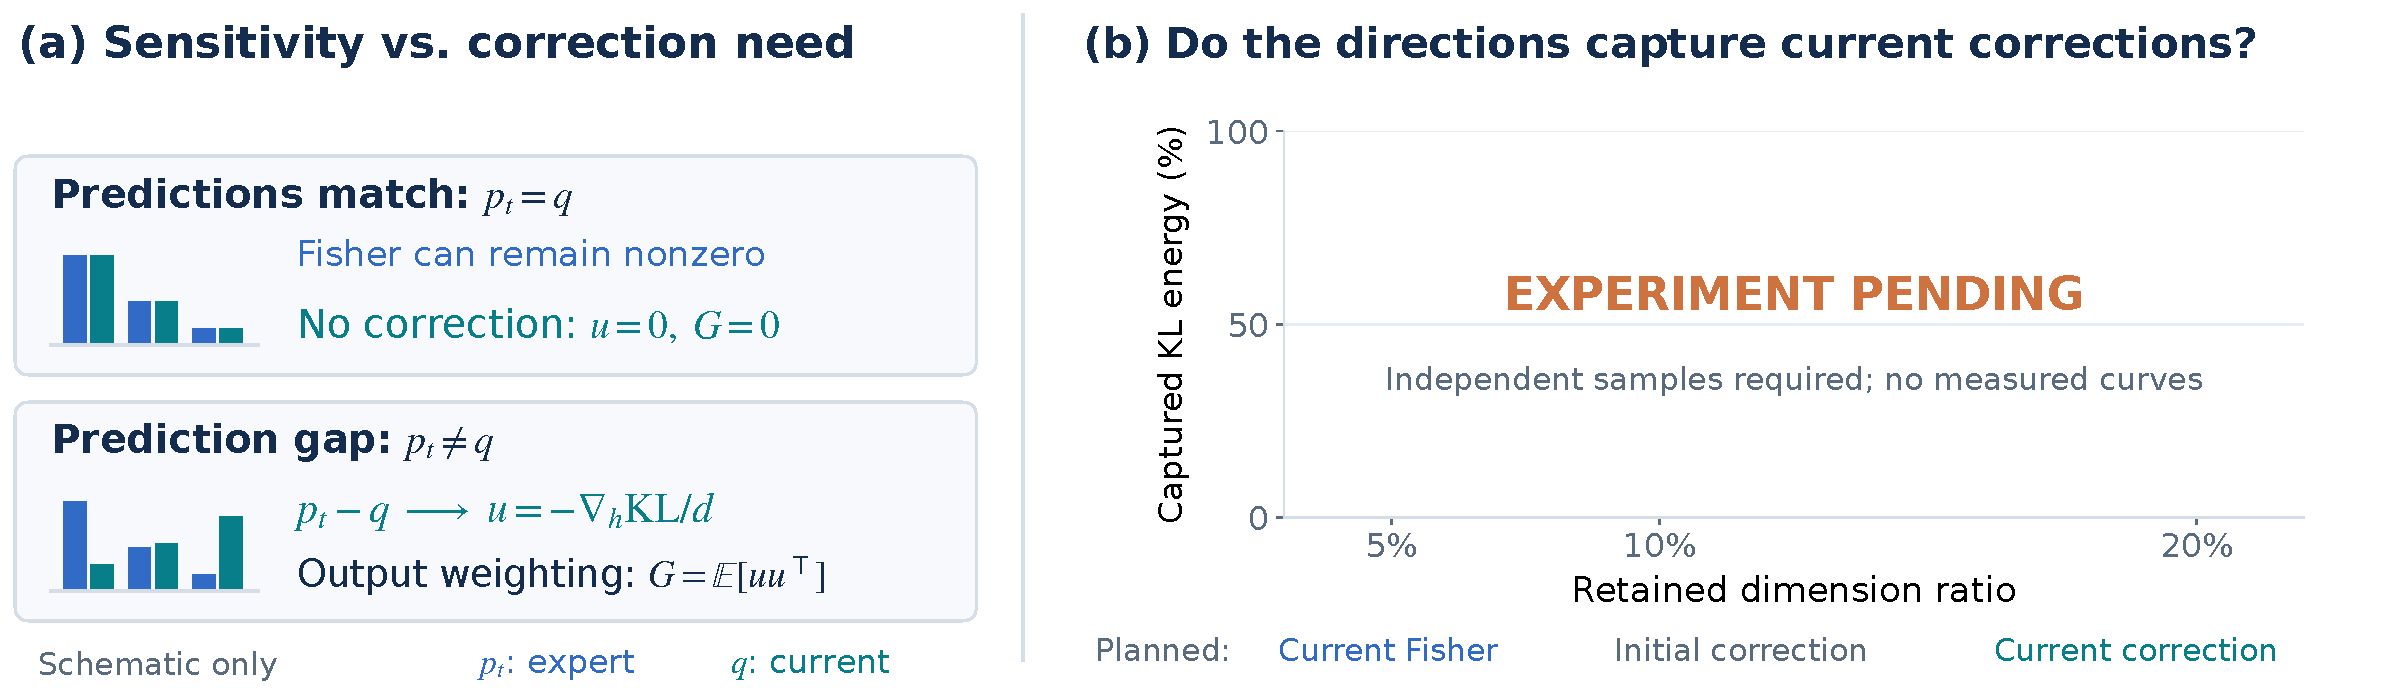
\includegraphics[width=\linewidth]{figures/ink_motivation.pdf}
  \caption{\textbf{局部敏感性不等于当前修正需求。}左：概念示意；当预测匹配时，Fisher 型几何仍可非零，而 KL 修正向量 $u$ 及其二阶矩 $G$ 为零；存在分歧时，残差经当前模型导数映射产生修正信号。右：独立样本修正能量捕获率的诊断版式，\textbf{实验待运行，无实测曲线}。此图不声称参数更新保证降低 KL。}
  \label{fig:ink-motivation}
\end{figure}

\section{相关工作}
\label{sec:ink-related-work}

\subsection{模型合并}

模型合并旨在将多个由同一预训练模型独立微调得到的专家模型整合为单一多任务模型，从而避免联合训练以及多模型推理带来的额外开销。早期方法主要在参数空间中进行组合，例如模型权重平均~\citep{wortsman2022model} 和任务向量算术~\citep{ilharco2023editing} 通过聚合专家参数更新实现知识融合。随后，研究逐渐关注不同任务更新之间的干扰问题，并从参数稀疏化、符号冲突以及任务子空间等角度提升合并效果。TIES-Merging 通过裁剪冗余更新并协调参数符号缓解任务间冲突~\citep{yadav2023ties}；TSV-M、Iso-C/CTS、WUDI-Merging 和 Essential Subspace Merging 等方法进一步利用任务更新的谱结构、共享子空间或任务特定子空间改善能力保留与组合~\citep{gargiulo2024task,marczak2025no,cheng2025whoever,li2026essential}。

除参数空间方法外，另一类工作利用额外信息自适应地调整合并过程。例如，AdaMerging 通过无标签数据上的熵优化学习任务级或层级合并系数~\citep{yang2024adamerging}。

\subsection{几何感知模型合并}

近年来，几何感知模型合并方法进一步将合并过程从简单参数距离扩展到任务相关几何空间，通过非各向同性度量区分不同参数方向的重要性。Fisher Merging 利用专家模型附近的 Fisher 信息刻画参数扰动对任务性能的影响~\citep{matena2022fisher}；RegMean 根据任务数据中的输入激活统计匹配不同模型的层输出，从而保留任务中频繁访问的输入方向~\citep{jin2023regmean}。MaTS 则将上述方法统一视为任务参数子空间中的模型匹配问题，并利用 Kronecker 分解和共轭梯度求解包含输入侧与输出侧结构的双侧线性系统~\citep{tam2024mats}。Chain of Merges 进一步考虑逐层合并过程中前序层变化导致的输入分布漂移，通过动态更新统计信息改善连续层之间的匹配~\citep{buzzega2025chain}。

这些方法的共同目标是通过任务相关几何判断哪些方向需要在合并过程中被保护。然而，它们所使用的几何通常来源于专家模型自身的参数统计、局部敏感性或任务数据分布。例如，RegMean 描述任务输入方向的覆盖程度，Fisher 和 MaTS 则描述专家附近参数扰动对任务目标的敏感程度。换言之，这些方法主要刻画专家模型中哪些方向具有重要性，但并不显式描述在当前合并模型下，为匹配某个专家仍需要修正哪些功能方向。

本文进一步将几何对象从固定的专家重要性几何扩展为动态的专家--当前模型修正几何。具体而言，\method{} 根据专家模型与当前合并模型之间的行为差异构造动态功能修正，并使该几何随着合并状态变化而重新估计。该方法从保护专家已有能力的重要方向，转向刻画当前模型为了接近专家仍需发生修正的功能方向。

\paragraph{与 MaTS 的详细比较。}
MaTS 用半正定矩阵 $C_t$ 表示专家 $t$ 的任务参数子空间，将合并写成
\begin{equation}
  \mathcal J_C(\theta)
  =
  \frac12\sum_{t=1}^T
  (\theta-\theta_t)^\top C_t(\theta-\theta_t),
  \qquad
  \left(\sum_tC_t\right)\theta^\star
  =
  \sum_tC_t\theta_t.
  \label{eq:ink-mats-subspace}
\end{equation}
对于线性层，K-FAC 近似令
\begin{equation}
  C_t^\ell\approx G_{t,F}^\ell\otimes A_t^\ell,
  \qquad
  G_{t,F}^\ell
  =
  \mathbb E\left[\delta_t^\ell(\delta_t^\ell)^\top\right],
\end{equation}
其中 $\delta_t^\ell$ 是任务损失对层输出的梯度。对应的双侧系统为
\begin{equation}
  \sum_tA_t^\ell X^\star G_{t,F}^\ell
  =
  \sum_tA_t^\ell X_t^\ell G_{t,F}^\ell.
  \label{eq:ink-mats-bilateral}
\end{equation}
Kronecker 乘积之和通常不能化为因子和的单个 Kronecker 乘积，因此 MaTS 将左侧视为线性算子，并用共轭梯度避免显式求逆。

\method{} 与 MaTS/K-FAC 在代数形式和求解器上最接近，但算子系数的语义与生命周期不同。MaTS 的 $G_{t,F}^\ell$ 是专家附近任务损失的输出梯度协方差，用固定任务子空间衡量哪些扰动敏感；\method{} 的 $G_{t,\mathrm{ink}}^{\ell,(r)}$ 则由专家--当前模型 KL 残差诱导，衡量当前模型尚需沿哪些功能方向修正，并在每次接受更新后改变。因此，我们复用的是双侧线性系统与共轭梯度这一计算骨架，而不是对同一个固定 Fisher 系统做更精确求解。

\section{问题设定}
\label{sec:ink-problem}

给定由同一预训练模型独立微调得到的 $T$ 个任务专家 $\{\theta_t\}_{t=1}^T$，记任务 $t$ 的无标签校准分布为 $\mathcal D_t$。对于输入 $x\sim\mathcal D_t$，专家 $t$ 给出有限类别分布
\begin{equation}
  p_t(c\mid x),
\end{equation}
而第 $r$ 轮合并模型 $\theta^{(r)}$ 给出
\begin{equation}
  q^{(r)}(c\mid x).
\end{equation}
不同任务可以使用不同的类别集合和任务头；待合并的是共享视觉编码器。我们仅要求在各自任务的数据上查询对应专家的软预测，不使用样本标签。

目标是使一个合并模型在每个任务上复现相应专家的预测行为：
\begin{equation}
  \mathcal L_t(\theta)
  =
  \mathbb E_{x\sim\mathcal D_t}
  \left[
    D_{\mathrm{KL}}
    \left(
      p_t(\cdot\mid x)
      \,\middle\|\,
      q_\theta(\cdot\mid x)
    \right)
  \right].
  \label{eq:ink-teacher-objective}
\end{equation}
校准样本用于估计合并几何，互不重叠的无标签留出样本用于选择更新步长和最终轮次。因而，问题不是直接决定一组固定的参数平均系数，而是估计：给定当前 $\theta^{(r)}$，每个专家还要求模型在哪些内部功能方向上发生改变。

\FloatBarrier
\flushbottom
\suppressfloats[t]
\section{\method{} 方法}
\label{sec:ink-functional-geometry}

\begin{figure}[!htbp]
  \centering
  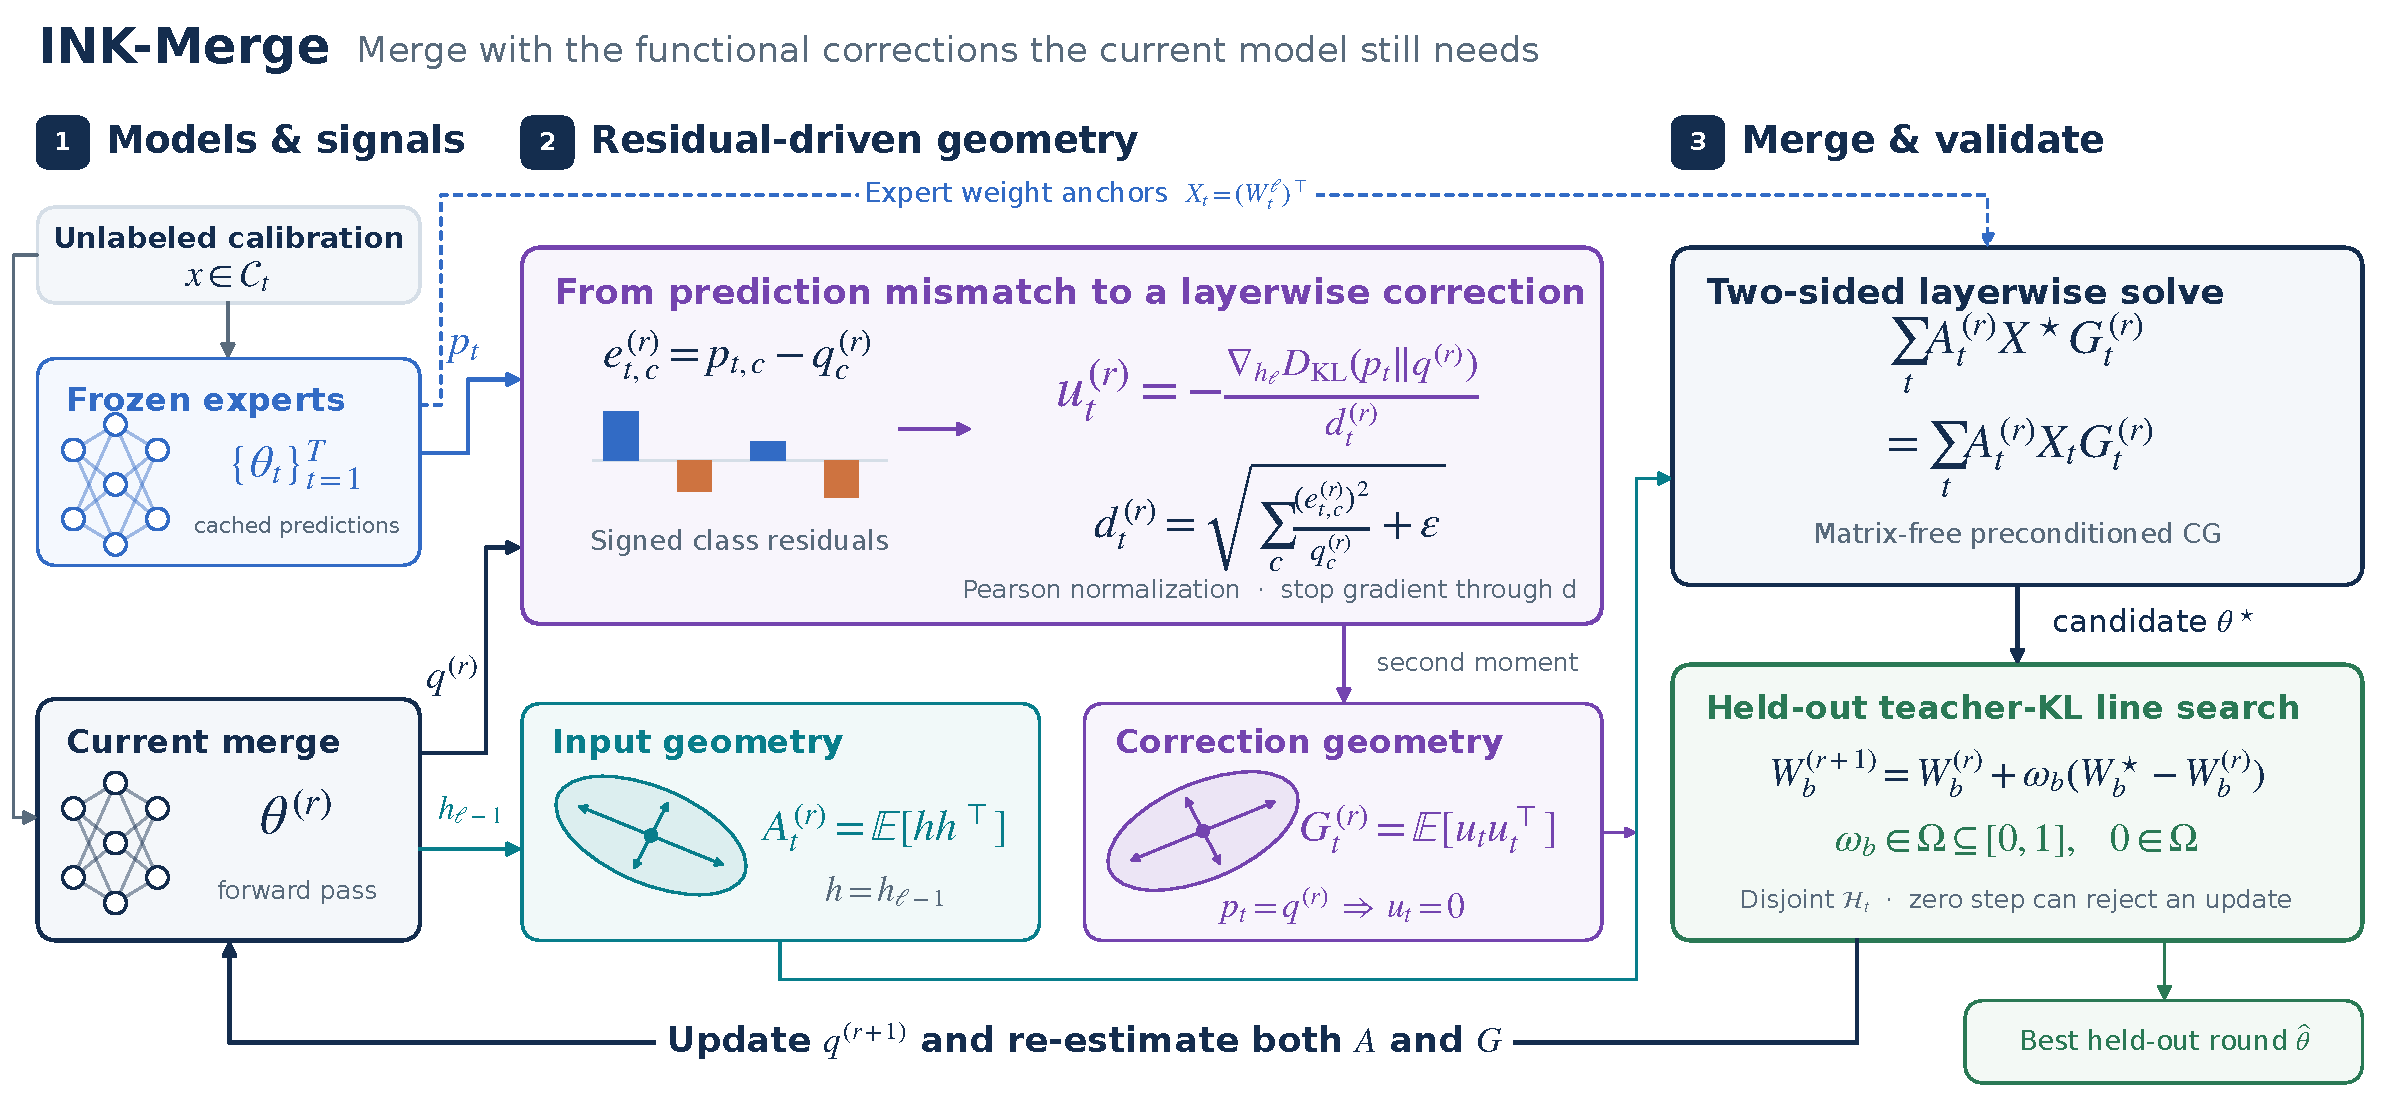
\includegraphics[width=\linewidth]{figures/ink_method_overview.pdf}
  \caption{\method{} 方法总览，对应式~(\ref{eq:ink-dynamic-geometry})。\textbf{1}~冻结专家提供软预测 $p_t$ 与权重锚点 $X_t$，当前模型 $\theta^{(r)}$ 给出 $q^{(r)}$ 与激活 $h_{\ell-1}$。\textbf{2}~类别残差经教师--学生 KL 负梯度与 Pearson 归一化得到层级修正 $u_t^{(r)}$；其二阶矩 $G_t^{(r)}$ 与输入二阶矩 $A_t^{(r)}$ 构成随 $\theta^{(r)}$ 变化的双侧几何。\textbf{3}~矩阵自由预条件共轭梯度求解候选权重，留出教师 KL 选择块级步长（含零步长拒绝），随后重估 $A$ 与 $G$ 并迭代，最终取留出 KL 最小的轮次。图中省略层下标 $\ell$，$G_t^{(r)}$ 简记 $G_{t,\mathrm{ink}}^{\ell,(r)}$，椭圆仅示意几何方向。}
  \label{fig:ink-overview}
\end{figure}


现有几何感知合并方法通常为每个专家估计固定的重要性几何 $C_t(\theta_t,\mathcal D_t)$。然而，模型更新后，它与不同专家之间尚未消除的功能差异也会改变，因此固定几何不能准确描述当前仍需保留或恢复的功能方向。\method{} 将几何写成式~(\ref{eq:ink-dynamic-geometry})，根据专家模型与当前合并模型之间的预测残差，在每一轮重新估计任务特定的功能修正几何。具体而言，我们将教师--学生 KL 关于层表示的归一化负梯度定义为局部功能修正向量，并以其二阶矩刻画输出侧几何。该几何与输入激活二阶矩共同构成 Kronecker 因子化度量，用于求解逐层参数合并。

\subsection{从预测残差到功能修正方向}

固定任务 $t$、输入 $x$ 和当前轮次 $r$，简写 $p_{t,c}=p_t(c\mid x)$、$q_c^{(r)}=q^{(r)}(c\mid x)$。首先定义专家与当前模型在类别 $c$ 上的预测残差
\begin{equation}
  e_{t,c}^{(r)}(x)
  =
  p_{t,c}-q_c^{(r)}.
  \label{eq:ink-prediction-residual}
\end{equation}
对第 $\ell$ 层表示 $h_\ell$，定义当前模型的类别得分
\begin{equation}
  s_c^{\ell,(r)}(x)
  =
  \nabla_{h_\ell}\log q^{(r)}(c\mid x).
\end{equation}
由于得分恒等式
\begin{equation}
  \sum_c q_c^{(r)}s_c^{\ell,(r)}(x)=0,
\end{equation}
教师--学生 KL 关于层表示的负梯度可以直接写为
\begin{align}
  -\nabla_{h_\ell}D_{\mathrm{KL}}(p_t\|q^{(r)})
  &= \sum_c p_{t,c}s_c^{\ell,(r)}(x) \\
  &= \sum_c \left(p_{t,c}-q_c^{(r)}\right)
     s_c^{\ell,(r)}(x).
  \label{eq:ink-kl-score-identity}
\end{align}
式~(\ref{eq:ink-kl-score-identity}) 将每个类别上的预测残差映射为层表示空间中的功能修正方向：$p_{t,c}>q_c^{(r)}$ 的类别沿其得分方向增强，$p_{t,c}<q_c^{(r)}$ 的类别则沿相反方向抵消。

\subsection{Pearson 归一化与局部修正}

为避免当前模型在某些类别上给出很小概率时产生过大的样本尺度，定义 Pearson 归一化项
\begin{equation}
  d_t^{(r)}(x)
  =
  \sqrt{
    \sum_c
    \frac{\left(p_{t,c}-q_c^{(r)}\right)^2}{q_c^{(r)}}
    +\varepsilon
  }.
  \label{eq:ink-pearson-normalizer}
\end{equation}
根号内除 $\varepsilon$ 外即为 $p_t$ 相对于 $q^{(r)}$ 的 Pearson-$\chi^2$ 散度。归一化的样本级修正向量为
\begin{align}
  u_t^{\ell,(r)}(x)
  &=
  \frac{
    \sum_c\left(p_{t,c}-q_c^{(r)}\right)
    s_c^{\ell,(r)}(x)
  }{d_t^{(r)}(x)} \\
  &=
  -\frac{
    \nabla_{h_\ell}D_{\mathrm{KL}}(p_t\|q^{(r)})
  }{d_t^{(r)}(x)}.
  \label{eq:ink-layer-correction}
\end{align}
该归一化保留各类别残差的相对符号与方向，同时使不同置信度尺度下的样本更可比较。实现时，我们对归一化教师 KL 做一次反向传播，并对分母停止梯度；反向钩子若收集到 $-u$，不会改变后续的 $uu^\top$。

\subsection{动态输出修正几何}

为了识别任务 $t$ 在不同样本上持续要求修正的功能子空间，定义输出侧二阶矩
\begin{equation}
  \boxed{
  G_{t,\mathrm{ink}}^{\ell,(r)}
  =
  \mathbb E_{x\sim\mathcal D_t}
  \left[
    u_t^{\ell,(r)}(x)u_t^{\ell,(r)}(x)^\top
  \right]
  }.
  \label{eq:ink-output-geometry}
\end{equation}
$G_{t,\mathrm{ink}}^{\ell,(r)}$ 为半正定矩阵，刻画任务 $t$ 在该层尚待修正方向的强度与相关结构。它同时依赖专家分布 $p_t$ 和当前分布 $q^{(r)}$：当两者匹配时，修正信号消失；当当前模型更新时，几何也随之改变。这与只描述专家附近局部敏感度的固定 Fisher 因子不同。

\subsection{Kronecker 因子化逐层合并}
\label{sec:ink-kronecker-merging}

考虑第 $\ell$ 个线性层。记专家 $t$ 的权重为 $W_t^\ell\in\mathbb R^{d_{\mathrm{out}}\times d_{\mathrm{in}}}$，并令 $X_t^\ell=(W_t^\ell)^\top$。输入侧几何由当前合并模型在任务数据上的激活二阶矩给出：
\begin{equation}
  A_t^{\ell,(r)}
  =
  \mathbb E_{x\sim\mathcal D_t}
  \left[h_{\ell-1}h_{\ell-1}^\top\right].
  \label{eq:ink-input-geometry}
\end{equation}
$A_t^{\ell,(r)}$ 描述该任务实际访问的输入方向，$G_{t,\mathrm{ink}}^{\ell,(r)}$ 描述尚未消除的输出功能分歧。二者定义双侧目标
\begin{equation}
  \mathcal J_\ell(X)
  =
  \frac12\sum_{t=1}^T
  \operatorname{tr}
  \left[
    (X-X_t^\ell)^\top
    A_t^{\ell,(r)}
    (X-X_t^\ell)
    G_{t,\mathrm{ink}}^{\ell,(r)}
  \right].
  \label{eq:ink-layer-objective}
\end{equation}
令梯度为零，得到正规方程
\begin{equation}
  \boxed{
  \sum_{t=1}^T
  A_t^{\ell,(r)}X^{\ell,\star}G_{t,\mathrm{ink}}^{\ell,(r)}
  =
  \sum_{t=1}^T
  A_t^{\ell,(r)}X_t^\ell G_{t,\mathrm{ink}}^{\ell,(r)}
  }.
  \label{eq:ink-normal-equation}
\end{equation}
我们把左侧实现为矩阵--矩阵线性算子，以对角预条件共轭梯度求解，不显式构造完整 Kronecker 矩阵。专家锚点 $X_t^\ell$ 保留参数目标位置；输出二阶矩虽把单个修正表示为功能轴，各类别预测残差的正负号已经在形成 $u$ 时决定不同得分方向如何增强或抵消。

\subsection{迭代重估与保守更新}
\label{sec:ink-iterative-update}

预测残差导出的功能修正、输入激活与输出修正几何都依赖当前模型。逐层求解式~(\ref{eq:ink-normal-equation}) 得到候选权重 $W^\star$ 后，对每个 Transformer 块采用保守插值
\begin{equation}
  W_b^{(r+1)}
  =
  W_b^{(r)}
  +
  \omega_b^{(r)}
  \left(W_b^\star-W_b^{(r)}\right),
  \qquad
  \omega_b^{(r)}\in\Omega\subseteq[0,1].
  \label{eq:ink-conservative-step}
\end{equation}
步长由互不重叠的无标签留出样本上的平均教师 KL 选择。候选集合始终包含 $0$，因此不能改善行为目标的块更新可以被完全拒绝。每轮接受后，算法围绕新的 $q^{(r+1)}$ 重新估计 $A_t^{\ell,(r+1)}$ 与 $G_{t,\mathrm{ink}}^{\ell,(r+1)}$；最终从初始化和所有轮次中选择留出教师 KL 最小者。

\begin{algorithm}[t]
  \DontPrintSemicolon
  \SetKwInput{KwIn}{输入}
  \SetKwInput{KwOut}{输出}
  \SetKw{KwTo}{至}
  \SetKwFor{For}{对于}{执行}{结束}
  \SetKwIF{If}{ElseIf}{Else}{如果}{则}{否则如果}{否则}{结束}
  \KwIn{专家 $\{\theta_t\}_{t=1}^T$；各任务无标签集合 $\{\mathcal C_t,\mathcal H_t\}$；轮数 $R$；步长 $\Omega$}
  \KwOut{合并模型 $\widehat\theta$}
  缓存每个专家在 $\mathcal C_t\cup\mathcal H_t$ 上的软预测 $p_t$\;
  以公共子空间合并初始化 $\theta^{(0)}$，并将其加入候选集 $\mathcal Q$\;
  \For{$r\leftarrow0$ \KwTo $R-1$}{
    在 $\theta^{(r)}$ 上计算 $q^{(r)}$、$A_t^{\ell,(r)}$ 和 $G_{t,\mathrm{ink}}^{\ell,(r)}$\;
    对每个线性层，以预条件共轭梯度求解式~(\ref{eq:ink-normal-equation})，得到 $W^{\ell,\star}$\;
    在 $\mathcal H_t$ 上以平均教师 KL 选择全局步长，并逐块细化 $\omega_b^{(r)}\in\Omega$\;
    按式~(\ref{eq:ink-conservative-step}) 得到 $\theta^{(r+1)}$，并加入 $\mathcal Q$\;
    \If{所有块的步长均为 $0$ 或相对更新量低于阈值}{停止}
  }
  $\widehat\theta\leftarrow\arg\min_{\theta\in\mathcal Q}\sum_t D_{\mathrm{KL}}(p_t\|q_\theta)$，其中 KL 在 $\mathcal H_t$ 上计算\;
  \caption{\method{} 的动态修正几何合并流程。}
  \label{alg:ink-merge}
\end{algorithm}


\subsection{与 MaTS 的关系}
\label{sec:ink-mats-comparison}

MaTS 用半正定矩阵 $C_t$ 表示专家 $t$ 的任务参数子空间，将合并写成
\begin{equation}
  \mathcal J_C(\theta)
  =
  \frac12\sum_{t=1}^T
  (\theta-\theta_t)^\top C_t(\theta-\theta_t),
  \qquad
  \left(\sum_tC_t\right)\theta^\star
  =
  \sum_tC_t\theta_t.
  \label{eq:ink-mats-subspace}
\end{equation}
对于线性层，K-FAC 近似令
\begin{equation}
  C_t^\ell\approx G_{t,F}^\ell\otimes A_t^\ell,
  \qquad
  G_{t,F}^\ell
  =
  \mathbb E\left[\delta_t^\ell(\delta_t^\ell)^\top\right],
\end{equation}
其中 $\delta_t^\ell$ 是任务损失对层输出的梯度。对应的双侧系统为
\begin{equation}
  \sum_tA_t^\ell X^\star G_{t,F}^\ell
  =
  \sum_tA_t^\ell X_t^\ell G_{t,F}^\ell.
  \label{eq:ink-mats-bilateral}
\end{equation}
Kronecker 乘积之和通常不能化为因子和的单个 Kronecker 乘积，因此 MaTS 将左侧视为线性算子，并用共轭梯度避免显式求逆。

\method{} 与 MaTS/K-FAC 在代数形式和求解器上最接近，但算子系数的语义与生命周期不同。MaTS 的 $G_{t,F}^\ell$ 是专家附近任务损失的输出梯度协方差，用固定任务子空间衡量哪些扰动敏感；\method{} 的 $G_{t,\mathrm{ink}}^{\ell,(r)}$ 则由专家--当前模型 KL 残差诱导，衡量当前模型尚需沿哪些功能方向修正，并在每次接受更新后改变。因此，我们复用的是双侧线性系统与共轭梯度这一计算骨架，而不是对同一个固定 Fisher 系统做更精确求解。

\section{实验设置}
\label{sec:ink-experiments}

\subsection{评估设置}

\paragraph{基准与指标。}
我们在 CLIP ViT-B/32~\citep{radford2021learning} 八任务基准上评估共享视觉编码器的合并，任务依次为 Cars、DTD、EuroSAT、GTSRB、MNIST、RESISC45、SVHN 和 SUN397。主指标是八个任务绝对测试准确率的无权算术平均。所有可调配置均只使用非测试划分选择；选定或冻结的模型在测试集上仅评估一次。

\paragraph{扩展骨干与语言模型。}
表~\ref{tab:ink-vision-summary} 按 ViT-B/32、ViT-B/16 和 ViT-L/14 分组，每组列出 8、14、20 tasks。当前只有 ViT-B/32 的 8 tasks 单元格有本地可核验记录，其余组合以 -- 预留。单元格主值为平均绝对准确率，括号内为逐任务相对独立专家准确率的平均值，即 $\frac{1}{T}\sum_t100\,\mathrm{Acc}_t/\mathrm{Acc}_{t,\mathrm{FT}}$。附录~\ref{apdx:ink-vitb32-details} 的表~\ref{tab:ink-vitb32-results} 给出已有八任务明细。

语言模型按所给参考表采用 Flan-T5-base，任务列为 CoLA、MNLI、MRPC、QNLI、QQP、RTE、SST2 和 STSB，并预留 ACC 汇总指标（表~\ref{tab:ink-t5-results}）。当前数字均为排版占位；持续合并顺序、指标计算、重复次数、合并模块和校准协议尚未从本地结果核验。以下实现细节与性能结论仅适用于已有的 ViT-B/32 冻结实验。

\subsection{实现细节}

\paragraph{数据划分与随机种子。}
每个任务从训练划分中缓存 512 个无标签样本，其中前 256 个用于统计估计，后 256 个作为互不重叠的留出集。附录表~\ref{tab:ink-vitb32-results} 报告随机种子 0 的主结果。我们还在不改变任何配置与候选步长的情况下使用种子 1 独立抽取验证/校准子集，并在相同冻结测试集上进行一次复核。

\paragraph{\method{} 配置。}
专家软预测在迭代前一次缓存；有限类别被精确枚举。合并模型以尺度 $1.3$ 的 Iso-C 初始化，最多执行 4 轮。每轮在当前模型上重估输入与输出统计，输入协方差不收缩，输出协方差使用自动 Ledoit--Wolf 收缩。式~(\ref{eq:ink-normal-equation}) 使用最多 100 步的对角预条件共轭梯度求解。全局和逐块线搜索都从
\begin{equation}
  \Omega=\{0,\,0.125,\,0.25,\,0.5,\,1\}
\end{equation}
中依据平均留出教师 KL 选择步长；精确平局偏向更小步长。实现取 $\varepsilon=10^{-8}$，相对更新停止阈值为 $10^{-8}$，并纳入 patch embedding 与输出投影等边界线性映射；非矩阵参数保持初始化值。轮次 0 也参与最终模型选择。

\subsection{比较方法}
参数空间和谱方法包括 Weight Avg.、Task Arithmetic~\citep{ilharco2023editing}、TIES~\citep{yadav2023ties}、Consensus TA~\citep{wang2024localizing}、Iso-C/CTS~\citep{marczak2025no}、TSV-M~\citep{gargiulo2024task}、WUDI~\citep{xiong2024adaptive}、LiNeS~\citep{wang2024lines}、ESM~\citep{li2026essential} 与 SVC~\citep{li2026spectral}；激活几何方法包括 RegMean~\citep{jin2023regmean} 和 Chain of Merges~\citep{buzzega2025chain}。

\section{实验结果}
\label{sec:ink-results}

\subsection{跨骨干与任务规模汇总}

\begin{table}[!htbp]
  \centering
  \caption{视觉模型合并汇总：三个骨干分别预留 8、14、20 tasks。单元格为平均绝对准确率$_{(\text{归一化准确率})}$（\%）；-- 表示本地缺少可核验结果。}
  \label{tab:ink-vision-summary}
  \setlength{\tabcolsep}{3.0pt}
  \renewcommand{\arraystretch}{1.15}
  \resizebox{\textwidth}{!}{%
  \begin{tabular}{@{}lccc|ccc|ccc@{}}
    \toprule
    \multirow{2}{*}{\textbf{Method}} &
    \multicolumn{3}{c}{\texttt{ViT-B-32}} &
    \multicolumn{3}{c}{\texttt{ViT-B-16}} &
    \multicolumn{3}{c}{\texttt{ViT-L-14}} \\
    \cmidrule(lr){2-4}\cmidrule(lr){5-7}\cmidrule(l){8-10}
    & 8 tasks & 14 tasks & 20 tasks & 8 tasks & 14 tasks & 20 tasks & 8 tasks & 14 tasks & 20 tasks \\
    \midrule
    Individual FT & $89.93_{(100.00)}$ & \placeholdervalue{--} & \placeholdervalue{--} & \placeholdervalue{--} & \placeholdervalue{--} & \placeholdervalue{--} & \placeholdervalue{--} & \placeholdervalue{--} & \placeholdervalue{--} \\
    \midrule
    Zero-shot & $46.69_{(53.63)}$ & \placeholdervalue{--} & \placeholdervalue{--} & \placeholdervalue{--} & \placeholdervalue{--} & \placeholdervalue{--} & \placeholdervalue{--} & \placeholdervalue{--} & \placeholdervalue{--} \\
    Weight Avg. & $66.42_{(73.83)}$ & \placeholdervalue{--} & \placeholdervalue{--} & \placeholdervalue{--} & \placeholdervalue{--} & \placeholdervalue{--} & \placeholdervalue{--} & \placeholdervalue{--} & \placeholdervalue{--} \\
    Task Arith. & $66.49_{(73.76)}$ & \placeholdervalue{--} & \placeholdervalue{--} & \placeholdervalue{--} & \placeholdervalue{--} & \placeholdervalue{--} & \placeholdervalue{--} & \placeholdervalue{--} & \placeholdervalue{--} \\
    TIES & $69.41_{(76.94)}$ & \placeholdervalue{--} & \placeholdervalue{--} & \placeholdervalue{--} & \placeholdervalue{--} & \placeholdervalue{--} & \placeholdervalue{--} & \placeholdervalue{--} & \placeholdervalue{--} \\
    Consensus TA & $70.36_{(77.86)}$ & \placeholdervalue{--} & \placeholdervalue{--} & \placeholdervalue{--} & \placeholdervalue{--} & \placeholdervalue{--} & \placeholdervalue{--} & \placeholdervalue{--} & \placeholdervalue{--} \\
    Iso-C & $81.33_{(90.21)}$ & \placeholdervalue{--} & \placeholdervalue{--} & \placeholdervalue{--} & \placeholdervalue{--} & \placeholdervalue{--} & \placeholdervalue{--} & \placeholdervalue{--} & \placeholdervalue{--} \\
    Iso-CTS & $81.04_{(89.86)}$ & \placeholdervalue{--} & \placeholdervalue{--} & \placeholdervalue{--} & \placeholdervalue{--} & \placeholdervalue{--} & \placeholdervalue{--} & \placeholdervalue{--} & \placeholdervalue{--} \\
    TSV-M & $81.35_{(90.08)}$ & \placeholdervalue{--} & \placeholdervalue{--} & \placeholdervalue{--} & \placeholdervalue{--} & \placeholdervalue{--} & \placeholdervalue{--} & \placeholdervalue{--} & \placeholdervalue{--} \\
    RegMean & $81.27_{(90.00)}$ & \placeholdervalue{--} & \placeholdervalue{--} & \placeholdervalue{--} & \placeholdervalue{--} & \placeholdervalue{--} & \placeholdervalue{--} & \placeholdervalue{--} & \placeholdervalue{--} \\
    WUDI & $82.55_{(91.37)}$ & \placeholdervalue{--} & \placeholdervalue{--} & \placeholdervalue{--} & \placeholdervalue{--} & \placeholdervalue{--} & \placeholdervalue{--} & \placeholdervalue{--} & \placeholdervalue{--} \\
    LiNeS (Iso-C) & $83.37_{(92.58)}$ & \placeholdervalue{--} & \placeholdervalue{--} & \placeholdervalue{--} & \placeholdervalue{--} & \placeholdervalue{--} & \placeholdervalue{--} & \placeholdervalue{--} & \placeholdervalue{--} \\
    CoM & $83.38_{(92.29)}$ & \placeholdervalue{--} & \placeholdervalue{--} & \placeholdervalue{--} & \placeholdervalue{--} & \placeholdervalue{--} & \placeholdervalue{--} & \placeholdervalue{--} & \placeholdervalue{--} \\
    ESM & $84.19_{(93.48)}$ & \placeholdervalue{--} & \placeholdervalue{--} & \placeholdervalue{--} & \placeholdervalue{--} & \placeholdervalue{--} & \placeholdervalue{--} & \placeholdervalue{--} & \placeholdervalue{--} \\
    SVC (Iso-CTS) & $81.61_{(90.79)}$ & \placeholdervalue{--} & \placeholdervalue{--} & \placeholdervalue{--} & \placeholdervalue{--} & \placeholdervalue{--} & \placeholdervalue{--} & \placeholdervalue{--} & \placeholdervalue{--} \\
    SVC (ESM) & $82.38_{(91.58)}$ & \placeholdervalue{--} & \placeholdervalue{--} & \placeholdervalue{--} & \placeholdervalue{--} & \placeholdervalue{--} & \placeholdervalue{--} & \placeholdervalue{--} & \placeholdervalue{--} \\
    \rowcolor{black!8}
    \textbf{\method{}} & $\boldsymbol{86.95_{(96.54)}}$ & \placeholdervalue{--} & \placeholdervalue{--} & \placeholdervalue{--} & \placeholdervalue{--} & \placeholdervalue{--} & \placeholdervalue{--} & \placeholdervalue{--} & \placeholdervalue{--} \\
    \bottomrule
  \end{tabular}%
  }
\end{table}


表~\ref{tab:ink-vision-summary} 将三个视觉骨干及三种任务规模合并为一张主表。ViT-B/32 的 8 tasks 一列保留已有复现记录，其他单元格为待补位置，不据此作规模扩展结论。

当前种子 0 的 \method{} 平均绝对准确率为 $86.95\%$，相对独立专家的归一化准确率为 $96.54\%$。其绝对准确率比 ESM、CoM 和 RegMean 分别高 $2.76$、$3.57$ 和 $5.67$ 个百分点，与 Individual FT 专家参考的差距为 $2.99$ 个百分点。

\FloatBarrier
\subsection{Flan-T5-base 持续模型合并}

\begin{table}[!htbp]
  \centering
  \caption{Flan-T5-base 八任务持续合并结果版式预留。所有灰色数字（含 $\pm$ 项）均为随机占位，非实测均值或标准差。}
  \label{tab:ink-t5-results}
  \setlength{\tabcolsep}{3.0pt}
  \renewcommand{\arraystretch}{1.18}
  \resizebox{\textwidth}{!}{%
  \begin{tabular}{@{}lrrrrrrrr|c@{}}
    \toprule
    \textbf{Method} & CoLA & MNLI & MRPC & QNLI & QQP & RTE & SST2 & STSB & ACC($\uparrow$) \\
    \midrule
    (Ref.) Single Fine-Tune & \placeholdervalue{71.8} & \placeholdervalue{90.9} & \placeholdervalue{67.1} & \placeholdervalue{83.1} & \placeholdervalue{82.8} & \placeholdervalue{81.0} & \placeholdervalue{91.1} & \placeholdervalue{85.6} & \placeholdervalue{$81.7\pm 1.3$} \\
    \midrule
    Zero-shot & \placeholdervalue{81.4} & \placeholdervalue{77.8} & \placeholdervalue{69.6} & \placeholdervalue{70.7} & \placeholdervalue{70.7} & \placeholdervalue{66.3} & \placeholdervalue{89.2} & \placeholdervalue{83.9} & \placeholdervalue{$76.2\pm 0.7$} \\
    Weight Avg. & \placeholdervalue{77.0} & \placeholdervalue{72.9} & \placeholdervalue{71.4} & \placeholdervalue{84.7} & \placeholdervalue{86.9} & \placeholdervalue{88.7} & \placeholdervalue{90.1} & \placeholdervalue{70.1} & \placeholdervalue{$80.2\pm 0.4$} \\
    Task Arith. & \placeholdervalue{92.0} & \placeholdervalue{73.0} & \placeholdervalue{71.0} & \placeholdervalue{72.1} & \placeholdervalue{73.2} & \placeholdervalue{67.4} & \placeholdervalue{87.4} & \placeholdervalue{80.1} & \placeholdervalue{$77.0\pm 0.7$} \\
    TIES & \placeholdervalue{75.0} & \placeholdervalue{74.0} & \placeholdervalue{73.8} & \placeholdervalue{67.4} & \placeholdervalue{66.4} & \placeholdervalue{72.4} & \placeholdervalue{81.2} & \placeholdervalue{65.7} & \placeholdervalue{$72.0\pm 0.2$} \\
    Consensus TA & \placeholdervalue{82.6} & \placeholdervalue{89.4} & \placeholdervalue{70.0} & \placeholdervalue{83.2} & \placeholdervalue{71.5} & \placeholdervalue{89.4} & \placeholdervalue{87.3} & \placeholdervalue{78.0} & \placeholdervalue{$81.4\pm 0.2$} \\
    Iso-C & \placeholdervalue{83.2} & \placeholdervalue{78.0} & \placeholdervalue{82.7} & \placeholdervalue{71.0} & \placeholdervalue{75.5} & \placeholdervalue{80.3} & \placeholdervalue{92.3} & \placeholdervalue{81.3} & \placeholdervalue{$80.5\pm 0.4$} \\
    Iso-CTS & \placeholdervalue{80.8} & \placeholdervalue{68.7} & \placeholdervalue{86.5} & \placeholdervalue{65.3} & \placeholdervalue{82.8} & \placeholdervalue{83.6} & \placeholdervalue{90.4} & \placeholdervalue{92.1} & \placeholdervalue{$81.3\pm 0.5$} \\
    TSV-M & \placeholdervalue{81.2} & \placeholdervalue{66.9} & \placeholdervalue{71.9} & \placeholdervalue{75.0} & \placeholdervalue{86.5} & \placeholdervalue{82.8} & \placeholdervalue{69.5} & \placeholdervalue{74.0} & \placeholdervalue{$76.0\pm 0.6$} \\
    RegMean & \placeholdervalue{82.2} & \placeholdervalue{72.4} & \placeholdervalue{68.2} & \placeholdervalue{89.2} & \placeholdervalue{91.6} & \placeholdervalue{88.2} & \placeholdervalue{92.8} & \placeholdervalue{74.7} & \placeholdervalue{$82.4\pm 0.1$} \\
    WUDI & \placeholdervalue{80.7} & \placeholdervalue{83.1} & \placeholdervalue{83.8} & \placeholdervalue{80.9} & \placeholdervalue{92.8} & \placeholdervalue{89.6} & \placeholdervalue{67.0} & \placeholdervalue{79.8} & \placeholdervalue{$82.2\pm 0.8$} \\
    LiNeS (Iso-C) & \placeholdervalue{87.3} & \placeholdervalue{77.9} & \placeholdervalue{68.1} & \placeholdervalue{67.3} & \placeholdervalue{67.0} & \placeholdervalue{74.1} & \placeholdervalue{66.9} & \placeholdervalue{76.1} & \placeholdervalue{$73.1\pm 0.5$} \\
    CoM & \placeholdervalue{70.2} & \placeholdervalue{65.6} & \placeholdervalue{88.4} & \placeholdervalue{65.0} & \placeholdervalue{91.9} & \placeholdervalue{87.4} & \placeholdervalue{82.1} & \placeholdervalue{74.0} & \placeholdervalue{$78.1\pm 1.4$} \\
    ESM & \placeholdervalue{82.5} & \placeholdervalue{92.2} & \placeholdervalue{91.0} & \placeholdervalue{84.8} & \placeholdervalue{76.2} & \placeholdervalue{84.6} & \placeholdervalue{77.0} & \placeholdervalue{66.9} & \placeholdervalue{$81.9\pm 0.2$} \\
    SVC (Iso-CTS) & \placeholdervalue{76.7} & \placeholdervalue{84.5} & \placeholdervalue{74.6} & \placeholdervalue{72.0} & \placeholdervalue{73.2} & \placeholdervalue{76.1} & \placeholdervalue{86.9} & \placeholdervalue{75.9} & \placeholdervalue{$77.5\pm 0.3$} \\
    SVC (ESM) & \placeholdervalue{86.5} & \placeholdervalue{76.6} & \placeholdervalue{92.2} & \placeholdervalue{89.9} & \placeholdervalue{65.7} & \placeholdervalue{83.6} & \placeholdervalue{90.8} & \placeholdervalue{70.6} & \placeholdervalue{$82.0\pm 1.2$} \\
    \rowcolor{black!8}
    \textbf{\method{} (Ours)} & \placeholdervalue{65.6} & \placeholdervalue{91.5} & \placeholdervalue{82.6} & \placeholdervalue{83.4} & \placeholdervalue{74.9} & \placeholdervalue{83.1} & \placeholdervalue{69.0} & \placeholdervalue{65.7} & \placeholdervalue{$77.0\pm 0.1$} \\
    \bottomrule
  \end{tabular}%
  }
  \par\smallskip
  {\footnotesize 随机占位 / 非实验结果。方法列表补齐视觉表基线；不沿用视觉结果。各方法的 T5 适配与持续合并实现、任务顺序、重复次数及 ACC 统计口径待核验。}
\end{table}


表~\ref{tab:ink-t5-results} 按参考表预留 Flan-T5-base 在八个任务上持续合并后的结果，并补齐视觉表中的方法列表。独立微调参考行置于顶部，Zero-shot 与各合并基线居中，\method{} 行以灰底突出。方法名称统一不表示其 T5 适配或持续合并版本已实现，也不沿用视觉实验的数值。所有数字及 $\pm$ 项均为排版占位，不代表已完成的运行、随机种子均值或标准差。正式实验记录补齐后，再按确认的任务顺序与指标协议填写 ACC 和逐任务表现。

\FloatBarrier
\subsection{种子复核}

逐任务明细见附录~\ref{apdx:ink-vitb32-details} 的表~\ref{tab:ink-vitb32-results}。

留出集轨迹与选择协议一致：种子 0 从轮次 0 的平均教师 KL $0.33332061$ 降至所选轮次 3 的 $0.15524809$，第 4 轮所有块步长均为零并停止。独立校准种子 1 在相同冻结配置下选择轮次 4，平均准确率为 $87.0496\%$，对应留出教师 KL 为 $0.13468810$。两个种子的平均准确率为 $86.9974\%$，总体标准差为 $0.0522$ 个百分点。该复核只衡量两次独立校准抽样下的稳定性，不替代更大规模的多种子评估。
\FloatBarrier

\subsection{输出几何收缩：稳定性与方向信息（待验证）}
\label{sec:ink-parameter-analysis}

以下三节将原参数图拆为独立分析。所有曲线均为\textbf{预期趋势示意，不是实验结果}；纵轴不提供准确率或 KL 数值，也不绘制虚构误差带。实际结果可能与这些假设不同。

\paragraph{要做什么。}
只扫描输出几何收缩强度，其余设置保持冻结协议不变。对非零输出二阶矩，先沿用实现的平均对角归一化得到 $\bar G$，再使用
\[
  G_\alpha=(1-\alpha)\bar G+\alpha I,\qquad
  \alpha\in\{0,0.1,\ldots,1.0\}.
\]
$\alpha=0$ 保留原方向结构，$\alpha=1$ 将非零输出度量变为单位矩阵；原始全零统计仍保持为零。输入几何不变更其收缩规则。现有逐任务、逐层自动收缩作为另一个完整配置单独运行，而不是人为对应到一个固定 $\alpha$。

\begin{figure}[!htbp]
  \centering
  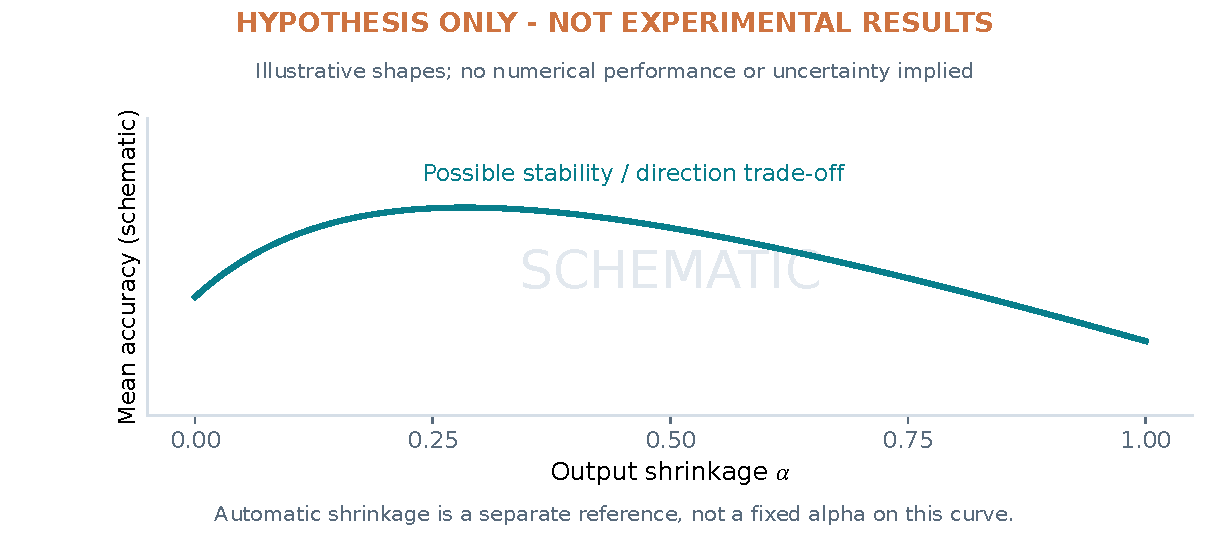
\includegraphics[width=0.78\linewidth]{figures/hypothesis_shrinkage.pdf}
  \caption{\textbf{输出收缩的预期趋势示意，非实验结果。}假设适度收缩能稳定有限样本的几何估计，而过强收缩会削弱方向信息；曲线可能存在宽缓的较优区间，但其形状和位置均待验证。纵轴无实测准确率刻度，自动收缩参照尚未绘制。}
  \label{fig:ink-parameter-analysis}
\end{figure}


\paragraph{如何解读。}
我们希望检验：轻度收缩是否有助于稳定有限样本估计，而强收缩是否丢失有用的输出方向信息。图~\ref{fig:ink-parameter-analysis} 画出一种可能的先升后降趋势，不是对最优 $\alpha$ 的预测。如果曲线平坦，就说明在该协议下对收缩不敏感；若单位度量不差，则不能据此声称输出方向信息不可替代。仅凭收缩曲线也不能分离方向结构和数值条件的全部影响。

\FloatBarrier
\subsection{统计样本量：多少无标签数据才够用（待验证）}
\label{sec:ink-sample-size-analysis}

\paragraph{要做什么。}
比较完整方法与每轮重估的当前模型 Fisher 对照。每个校准种子先固定统计样本顺序，再取前 32、64、128、256 个构成嵌套子集；两种方法在每个样本量下使用完全相同的子集。留出集始终是另外同一组 256 个样本，不能随着统计样本量缩小，也不能与统计子集重叠。每个设置从相同初始化独立运行完整合并流程，不能沿用上一个样本量的已合并权重。除样本量和输出几何类型外，求解预算、自动收缩规则、步长选择及轮次上限均相同。

\begin{figure}[!htbp]
  \centering
  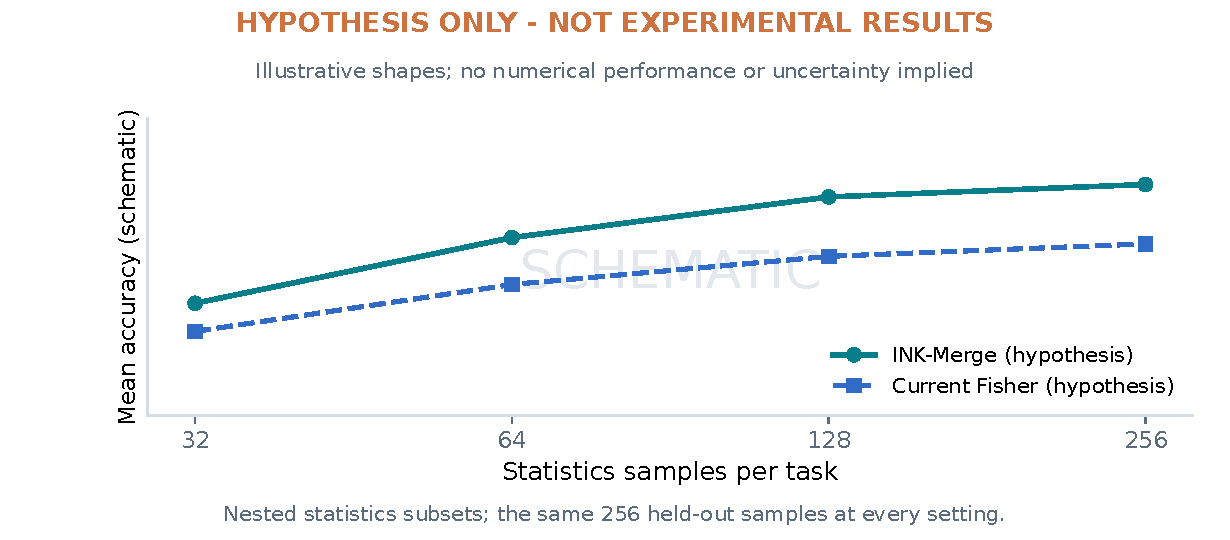
\includegraphics[width=0.78\linewidth]{figures/hypothesis_samples.pdf}
  \caption{\textbf{统计样本量的预期趋势示意，非实验结果。}待验证假设是样本增加带来收益递减，修正几何可能在有限样本下优于当前 Fisher。曲线间距和拐点仅供解释，既不是测得的性能差值，也不证明 128 或 256 个样本已经足够。}
  \label{fig:ink-sample-size-analysis}
\end{figure}


\paragraph{如何解读。}
图~\ref{fig:ink-sample-size-analysis} 示意的假设是：样本更多时估计更稳定，平均准确率逐渐提高并趋于饱和；修正几何可能在小样本区间更有效。需要用真实数据判断曲线是否饱和、两种方法的差异是否跨种子一致，不能从示意图认定某个样本数已足够。横轴只计统计样本，实际无标签数据预算还包括固定的 256 个留出样本；512 或 1024 个统计样本需另备数据，不能从留出集挪用。

\FloatBarrier
\subsection{迭代重估：动态输出几何是否必要（待验证）}
\label{sec:ink-iteration-analysis}

\paragraph{要做什么。}
从同一初始化分别运行三组对照：每轮重估当前模型 Fisher；固定初始输出修正几何 $G^{(0)}$、但持续重估输入几何 $A$；完整方法同时重估 $A,G$。在每个变体各自的轨迹上记录第 0--4 轮状态，并用同一独立诊断集计算八任务等权平均教师 KL。该诊断集不得参与几何估计、步长或轮次选择；所有对照使用相同统计和留出划分。现有固定首轮统计开关会同时冻结 $A,G$，不能直接用来实现第二组对照。

\begin{figure}[!htbp]
  \centering
  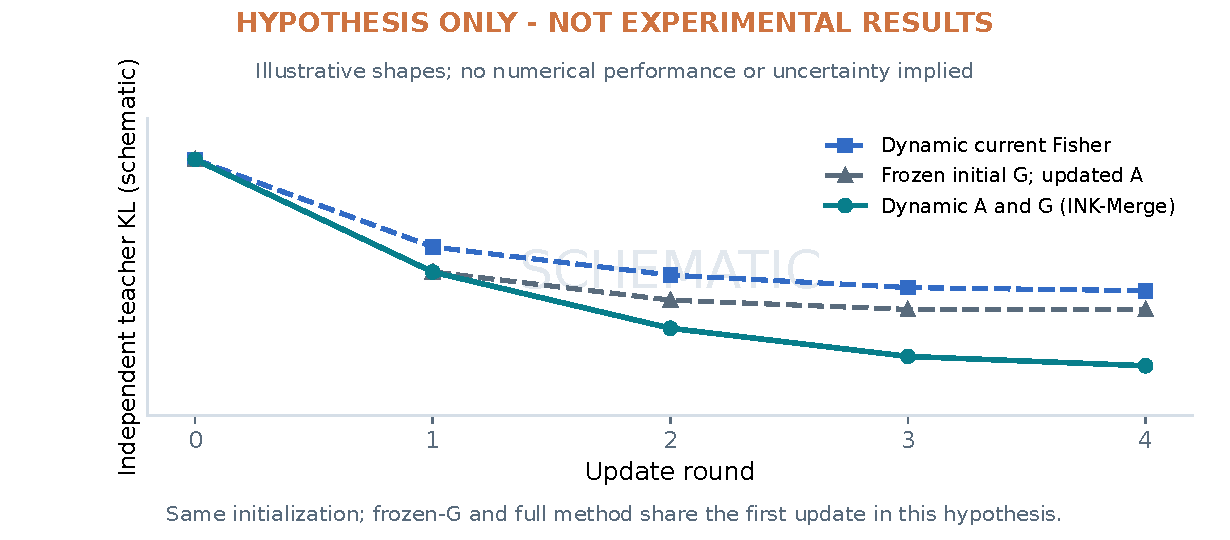
\includegraphics[width=0.78\linewidth]{figures/hypothesis_rounds.pdf}
  \caption{\textbf{动态性对照的预期趋势示意，非实验结果。}三种设置共享初始化；仅冻结初始 $G$ 与完整方法在相同协议下共享第一轮候选更新，差异应在后续重估中体现。图示假设动态修正几何可继续降低独立 KL，不表示真实曲线必然单调或方法排名已确定。}
  \label{fig:ink-iteration-analysis}
\end{figure}


\paragraph{如何解读。}
图~\ref{fig:ink-iteration-analysis} 中仅冻结 $G$ 与完整方法的首轮更新重合：此时两者都使用相同的初始几何。后续若完整方法持续优于冻结 $G$，才支持重估输出几何的价值；若优于动态 Fisher，才支持残差条件化在该设置下的价值。独立 KL 可能回升，不要求单调下降。提前停止时只报告已完成轮次，或将保持不变的尾段明确标注为停止后的状态延续，不伪装成新更新。

\paragraph{共同评估约束。}
上述扫描固定使用校准种子 0、1、2；真实结果分别保存每种子的曲线，再报告均值与样本标准差。当前仅有两个种子的冻结记录，不足以补齐这些实验。所有配置、数据划分和扫描点在运行前固定；测试准确率只用于最终诊断报告，不用于反选默认参数、轮次或步长。既有留出 KL 轨迹仅说明选择过程，不能替代独立诊断。前面的图~\ref{fig:ink-motivation} 仍单独负责修正能量的机制诊断。

\FloatBarrier
\subsection{核心设计消融（待运行）}
\label{sec:ink-core-ablation}

\begin{table}[!htbp]
  \centering
  \caption{核心设计消融表位。\textbf{全部待运行}；-- 表示缺少同协议实验结果，完整方法也需在相同的新种子协议下运行，不将现有两种子结果拼入本表。}
  \label{tab:ink-core-ablation}
  \small
  \setlength{\tabcolsep}{4pt}
  \renewcommand{\arraystretch}{1.35}
  \begin{tabularx}{\linewidth}{@{}X X cc@{}}
    \toprule
    对照 & 验证问题 & 平均准确率 $\uparrow$ & 诊断 KL $\downarrow$ \\
    \midrule
    \rowcolor{black!8}
    完整 \method{} & 同协议参考 & -- & -- \\
    当前 Fisher 替换修正 $G$ & 残差条件化 & -- & -- \\
    仅固定 $G^{(0)}$，更新 $A$ & 动态输出几何 & -- & -- \\
    去掉 Pearson 归一化 & 样本尺度控制 & -- & -- \\
    仅做全局线搜索 & 逐块步长选择 & -- & -- \\
    每轮完整采用候选更新 & 保守更新 & -- & -- \\
    \bottomrule
  \end{tabularx}
\end{table}


表~\ref{tab:ink-core-ablation} 预留六组对照，各组保持统计样本、留出样本、初始化、求解预算与收缩规则可比，未来报告至少三个相同校准种子下的均值与标准差。仅全局线搜索的变体关闭逐块精调；完整候选更新的变体则每轮直接接受候选权重，不依据留出 KL 拒绝该轮更新。后者需要专门实现并验证，不能把要求包含零的现有步长候选接口简单设成 $\{1\}$。所有新变体结果目前均为空，未改变正文已有的冻结实验结论。

单轮 0--1 步长诊断、初始化依赖和求解成本图位分别见附录~\ref{apdx:ink-step-size}、\ref{apdx:ink-initialization}、\ref{apdx:ink-cost}。若计算预算有限，优先级为核心消融表、输出收缩扫描、统计样本量扫描。
\FloatBarrier

\FloatBarrier
\section{结论}
\label{sec:ink-conclusion}

本文提出 \method{}，根据专家与当前合并模型之间尚未消除的预测残差，动态识别每一层需要修正的功能方向。教师--学生 KL 关于层表示的归一化负梯度给出局部修正，其二阶矩与当前输入激活几何共同形成 Kronecker 因子化正规方程，并由共轭梯度、逐块保守步长和留出教师 KL 完成迭代合并。冻结的 CLIP ViT-B/32 八任务实验表明，该方法在两个独立校准种子下分别取得 $86.95\%$ 和 $87.05\%$ 的平均准确率。

当前结论限定于可精确枚举类别、具有每任务无标签校准样本的 CLIP 视觉基准。进一步验证仍需覆盖更多架构、任务规模与随机种子，并评估校准数据需求和迭代统计重估的计算代价。


\bibliography{references}
\bibliographystyle{iclr2023_conference}

\appendix
\section{ViT-B/32 八任务逐任务明细}
\label{apdx:ink-vitb32-details}

表~\ref{tab:ink-vitb32-results} 给出 CLIP ViT-B/32 八任务基准上各方法的逐任务测试准确率，作为正文表~\ref{tab:ink-vision-summary} 中该列平均值的展开。粗体和下划线分别标记所列合并记录中的最优与次优。

\begin{table}[!htbp]
  \centering
  \caption{CLIP ViT-B/32 八任务逐任务明细（\%）。粗体和下划线分别标记所列合并记录中的最优与次优。Individual FT 为独立专家参考。}
  \label{tab:ink-vitb32-results}
  \setlength{\tabcolsep}{2.4pt}
  \renewcommand{\arraystretch}{1.04}
  \resizebox{\textwidth}{!}{%
  \begin{tabular}{@{}lrrrrrrrrr@{}}
    \toprule
    方法 & Cars & DTD & EuroSAT & GTSRB & MNIST & RESISC45 & SVHN & SUN397 & 平均 \\
    \midrule
    Zero-shot & 56.54 & 41.91 & 39.15 & 32.81 & 53.91 & 57.94 & 28.77 & 62.51 & 46.69 \\
    Weight Avg. & 58.86 & 48.35 & 65.78 & 64.94 & 92.42 & 67.97 & 72.80 & 60.21 & 66.42 \\
    Task Arith. & 57.74 & 48.03 & 66.48 & 66.52 & 93.69 & 66.67 & 74.46 & 58.34 & 66.49 \\
    TIES & 59.68 & 50.16 & 65.04 & 70.42 & 97.22 & 70.41 & 82.91 & 59.44 & 69.41 \\
    Consensus TA & 58.99 & 51.44 & 71.04 & 73.56 & 97.37 & 68.75 & 83.19 & 58.52 & 70.36 \\
    Iso-C & 70.00 & 65.37 & 88.33 & 90.74 & 98.82 & 84.68 & 86.72 & 65.95 & 81.33 \\
    Iso-CTS & 69.32 & 65.53 & 88.81 & 91.07 & 98.84 & 84.90 & 84.93 & 64.92 & 81.04 \\
    TSV-M & 68.86 & 64.73 & 91.19 & 90.95 & 99.11 & 81.81 & 89.89 & 64.24 & 81.35 \\
    RegMean & 66.87 & 64.15 & 93.41 & 87.71 & 98.31 & 82.29 & 91.22 & 66.23 & 81.27 \\
    WUDI & 68.23 & 65.90 & 94.11 & 92.45 & \textbf{99.31} & 82.10 & 92.86 & 65.44 & 82.55 \\
    LiNeS (Iso-C) & 72.91 & 69.31 & 92.33 & 92.56 & 99.10 & 86.73 & 86.87 & 67.14 & 83.37 \\
    CoM & 67.14 & 66.65 & \underline{95.26} & 91.70 & 98.93 & 85.17 & \underline{94.76} & 67.41 & 83.38 \\
    ESM & 73.27 & \underline{71.44} & 91.04 & \underline{93.17} & \underline{99.30} & \underline{88.24} & 90.48 & 66.55 & \underline{84.19} \\
    SVC (Iso-CTS) & 72.29 & 67.45 & 88.81 & 89.59 & 98.24 & 85.51 & 81.65 & \underline{69.32} & 81.61 \\
    SVC (ESM) & \textbf{74.00} & 65.96 & 89.74 & 88.72 & 98.92 & 85.02 & 87.62 & 69.09 & 82.38 \\
    \midrule
    \textbf{\method{}} & \underline{73.91} & \textbf{71.76} & \textbf{97.44} & \textbf{96.27} & 99.23 & \textbf{90.03} & \textbf{95.91} & \textbf{71.01} & \textbf{86.95} \\
    \midrule
    Individual FT（上界） & 76.30 & 77.71 & 99.89 & 99.10 & 99.70 & 95.48 & 97.51 & 73.79 & 89.93 \\
    \bottomrule
  \end{tabular}%
  }
\end{table}


在所列合并记录中，\method{} 在 DTD、EuroSAT、GTSRB、RESISC45、SVHN 和 SUN397 的数值最高，Cars 次高，MNIST 低于 WUDI 和 ESM。

\FloatBarrier
\section{单轮更新步长诊断（待验证）}
\label{apdx:ink-step-size}

本节将准确率与 KL 拆为两个独立小节和图，说明为什么几何目标的候选解未必适合直接完整替换当前权重。\textbf{以下曲线仅为可能趋势，不是实测结果}，两图的纵轴均无数值刻度。

\paragraph{先固定同一个候选方向。}
对每个预先固定的校准种子，只从初始化模型估计一次第一轮几何、求解一次候选权重 $W^\star$，然后构造
\[
  W(\omega)=W^{(0)}+\omega\bigl(W^\star-W^{(0)}\bigr),\qquad
  \omega\in\{0,0.1,\ldots,1.0\}.
\]
每个 $\omega$ 都从同一 $W^{(0)}$ 插值，不能在上一个步长的模型上累计更新。扫描期间不重新估计几何、不执行逐块精调；非合并参数保持初始化值。$\omega=0$ 是当前 Iso-C 初始化而非 Zero-shot，$\omega=1$ 才是完整采用第一轮候选解。

\subsection{步长对准确率的影响}
\paragraph{要做什么。}
对上述 11 个模型，在预先固定的测试协议下计算八任务等权平均准确率。未来对每个种子记录原留出 KL 在原候选集合中选出的全局步长，分别标注而不把多个种子的位置平均成一个实际步长。若该步长不在 0.1 间隔网格内，可额外评价其模型，但不得据测试结果重新选步。

\begin{figure}[!htbp]
  \centering
  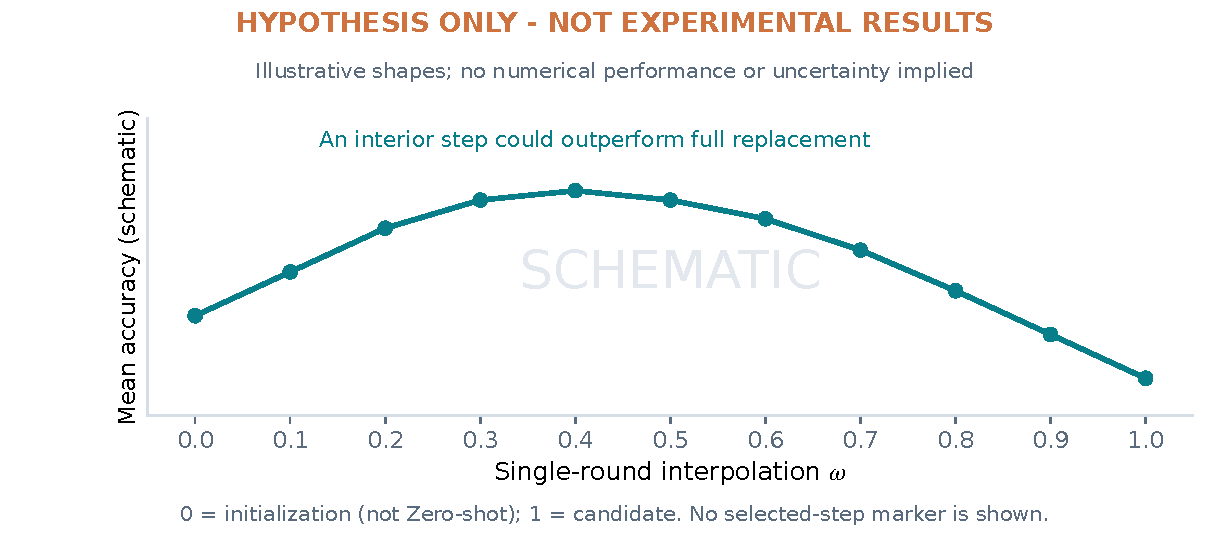
\includegraphics[width=0.78\linewidth]{figures/hypothesis_step_accuracy.pdf}
  \caption{\textbf{单轮步长--准确率的预期趋势示意，非实验结果。}可能的情形是中间步长优于完整替换；示意峰值不对应推荐步长。$\omega=0$ 为初始化模型而非 Zero-shot，$\omega=1$ 为完整候选更新。图中没有实际选步标记。}
  \label{fig:ink-step-size-analysis}
\end{figure}


\paragraph{如何解读。}
图~\ref{fig:ink-step-size-analysis} 示意一种可能的先升后降关系：适度更新恢复任务功能，而完整替换可能过度改变当前模型。若真实 $\omega=1$ 反而最好，则不能用该轮准确率支持保守更新；若多数步长都差，也需检查候选方向本身。图中的峰值位置完全是画图示意，不代表建议使用 $0.4$，也不是完整多轮、逐块 \method{} 的结果。

\clearpage
\subsection{步长对教师 KL 的影响}
\paragraph{要做什么。}
保持上一小节的模型集合不变，在未参与统计、步长与轮次选择的独立诊断集上计算教师--学生 KL，先按任务平均，再对八个任务等权平均。原留出 KL 选步只是标注对象，不能改由独立诊断集或测试集选择。本图与准确率图分开作图，不使用双纵轴。

\begin{figure}[!htbp]
  \centering
  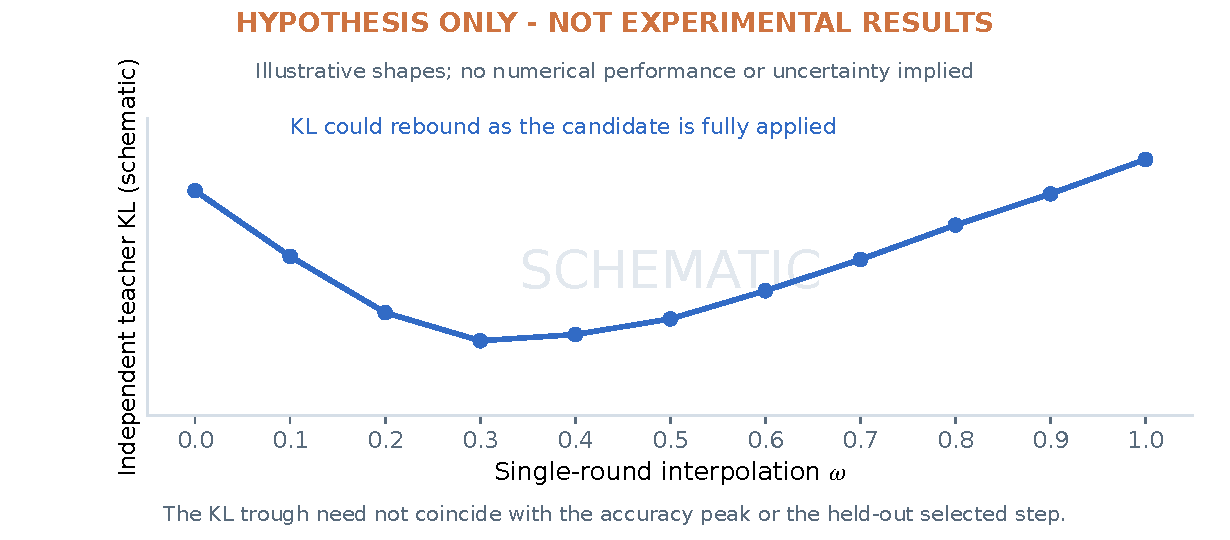
\includegraphics[width=0.78\linewidth]{figures/hypothesis_step_kl.pdf}
  \caption{\textbf{单轮步长--教师 KL 的预期趋势示意，非实验结果。}可能的情形是 KL 随小步更新降低、随后回升；不保证回升一定出现，也不保证最低点与图~\ref{fig:ink-step-size-analysis} 的准确率峰值重合。纵轴无实测 KL 数值，原留出集选步需待运行后另行标注。}
  \label{fig:ink-step-kl-analysis}
\end{figure}


\paragraph{如何解读。}
图~\ref{fig:ink-step-kl-analysis} 示意小步降低 KL、较大步长发生回升的可能情形。几何目标中的专家参数锚点与 Kronecker 近似并不等同于直接最小化真实教师 KL，因此完整候选更新未必最优。但真实 KL 也可能单调下降；即使出现中间最低点，也只能支持该候选方向在这些样本上的局部诊断，不能证明普遍最优步长。

准确率涉及真实标签，KL 衡量对专家分布的匹配，二者的最优位置不必一致；原留出集与独立诊断集的最低点也不必一致。示意图特意没有让两图的拐点重合，并且未绘制任何实际选步标线。正式实验沿用种子 0、1、2，报告真实曲线及差异；完整线搜索的多轮贡献仍需正文表~\ref{tab:ink-core-ablation} 的消融检验。

\clearpage
\section{初始化依赖（待运行）}
\label{apdx:ink-initialization}

\begin{figure}[!htbp]
  \centering
  \begin{minipage}[t]{0.485\linewidth}
    \analysisplotslot{0.15\textheight}{(a) Iso-C 初始化尺度}{1.3 附近；扫描点待预注册}{平均准确率（\%）}
  \end{minipage}\hfill
  \begin{minipage}[t]{0.485\linewidth}
    \analysisplotslot{0.15\textheight}{(b) 不同初始化}{初始化方法；列表待预注册}{平均准确率（\%）}
  \end{minipage}
  \caption{初始化依赖图位，\textbf{待运行}。左侧考察当前 Iso-C 尺度 $1.3$ 附近的设置，右侧预留其他初始化对照；扫描范围和初始化列表在运行前固定，不能由测试曲线反选默认值。}
  \label{fig:ink-initialization-analysis}
\end{figure}


预留 Iso-C 尺度 $1.3$ 附近及不同初始化方法的两组诊断。正式运行前固定候选列表、随机种子和相同的数据划分，除初始化外保持合并及选择协议一致；当前没有初始化扫描结果，不以现有单点表现推断稳健范围。

\FloatBarrier
\section{求解预算与计算成本（待运行）}
\label{apdx:ink-cost}

\begin{figure}[!htbp]
  \centering
  \begin{minipage}[t]{0.32\linewidth}
    \analysisplotslot{0.15\textheight}{(a) CG 求解预算}{最大 CG 步数}{平均准确率（\%）}
  \end{minipage}\hfill
  \begin{minipage}[t]{0.32\linewidth}
    \analysisplotslot{0.15\textheight}{(b) 时间成本}{最大 CG 步数}{合并耗时（秒）}
  \end{minipage}\hfill
  \begin{minipage}[t]{0.32\linewidth}
    \analysisplotslot{0.15\textheight}{(c) 显存成本}{最大 CG 步数}{峰值显存（GiB）}
  \end{minipage}
  \caption{求解预算与成本分析图位，\textbf{待运行}。三面板使用同一组预注册 CG 预算、相同硬件和批量设置，报告实际迭代次数、停止容差与计时范围；不把未测量的耗时或显存填为估算结果。}
  \label{fig:ink-cost-analysis}
\end{figure}


预留 CG 预算对准确率、合并耗时及峰值显存的影响。扫描点与是否包含专家预测缓存、几何统计和线搜索的计时边界须在运行前固定；所有设置使用相同设备、精度、批量和数据。记录最大与实际 CG 步数、残差容差及至少三个校准种子的统计，不将跨设备记录直接视为算法成本差异。

\FloatBarrier


\end{document}
